\documentclass[]{article}
\usepackage{lmodern}
\usepackage{amssymb,amsmath}
\usepackage{ifxetex,ifluatex}
\usepackage{fixltx2e} % provides \textsubscript
\ifnum 0\ifxetex 1\fi\ifluatex 1\fi=0 % if pdftex
  \usepackage[T1]{fontenc}
  \usepackage[utf8]{inputenc}
\else % if luatex or xelatex
  \ifxetex
    \usepackage{mathspec}
    \usepackage{xltxtra,xunicode}
  \else
    \usepackage{fontspec}
  \fi
  \defaultfontfeatures{Mapping=tex-text,Scale=MatchLowercase}
  \newcommand{\euro}{€}
\fi
% use upquote if available, for straight quotes in verbatim environments
\IfFileExists{upquote.sty}{\usepackage{upquote}}{}
% use microtype if available
\IfFileExists{microtype.sty}{%
\usepackage{microtype}
\UseMicrotypeSet[protrusion]{basicmath} % disable protrusion for tt fonts
}{}
\usepackage[margin=1in]{geometry}
\usepackage{color}
\usepackage{fancyvrb}
\newcommand{\VerbBar}{|}
\newcommand{\VERB}{\Verb[commandchars=\\\{\}]}
\DefineVerbatimEnvironment{Highlighting}{Verbatim}{commandchars=\\\{\}}
% Add ',fontsize=\small' for more characters per line
\usepackage{framed}
\definecolor{shadecolor}{RGB}{248,248,248}
\newenvironment{Shaded}{\begin{snugshade}}{\end{snugshade}}
\newcommand{\KeywordTok}[1]{\textcolor[rgb]{0.13,0.29,0.53}{\textbf{{#1}}}}
\newcommand{\DataTypeTok}[1]{\textcolor[rgb]{0.13,0.29,0.53}{{#1}}}
\newcommand{\DecValTok}[1]{\textcolor[rgb]{0.00,0.00,0.81}{{#1}}}
\newcommand{\BaseNTok}[1]{\textcolor[rgb]{0.00,0.00,0.81}{{#1}}}
\newcommand{\FloatTok}[1]{\textcolor[rgb]{0.00,0.00,0.81}{{#1}}}
\newcommand{\CharTok}[1]{\textcolor[rgb]{0.31,0.60,0.02}{{#1}}}
\newcommand{\StringTok}[1]{\textcolor[rgb]{0.31,0.60,0.02}{{#1}}}
\newcommand{\CommentTok}[1]{\textcolor[rgb]{0.56,0.35,0.01}{\textit{{#1}}}}
\newcommand{\OtherTok}[1]{\textcolor[rgb]{0.56,0.35,0.01}{{#1}}}
\newcommand{\AlertTok}[1]{\textcolor[rgb]{0.94,0.16,0.16}{{#1}}}
\newcommand{\FunctionTok}[1]{\textcolor[rgb]{0.00,0.00,0.00}{{#1}}}
\newcommand{\RegionMarkerTok}[1]{{#1}}
\newcommand{\ErrorTok}[1]{\textbf{{#1}}}
\newcommand{\NormalTok}[1]{{#1}}
\usepackage{graphicx}
\makeatletter
\def\maxwidth{\ifdim\Gin@nat@width>\linewidth\linewidth\else\Gin@nat@width\fi}
\def\maxheight{\ifdim\Gin@nat@height>\textheight\textheight\else\Gin@nat@height\fi}
\makeatother
% Scale images if necessary, so that they will not overflow the page
% margins by default, and it is still possible to overwrite the defaults
% using explicit options in \includegraphics[width, height, ...]{}
\setkeys{Gin}{width=\maxwidth,height=\maxheight,keepaspectratio}
\ifxetex
  \usepackage[setpagesize=false, % page size defined by xetex
              unicode=false, % unicode breaks when used with xetex
              xetex]{hyperref}
\else
  \usepackage[unicode=true]{hyperref}
\fi
\hypersetup{breaklinks=true,
            bookmarks=true,
            pdfauthor={},
            pdftitle={R: lo básico},
            colorlinks=true,
            citecolor=blue,
            urlcolor=blue,
            linkcolor=magenta,
            pdfborder={0 0 0}}
\urlstyle{same}  % don't use monospace font for urls
\setlength{\parindent}{0pt}
\setlength{\parskip}{6pt plus 2pt minus 1pt}
\setlength{\emergencystretch}{3em}  % prevent overfull lines
\setcounter{secnumdepth}{5}

%%% Use protect on footnotes to avoid problems with footnotes in titles
\let\rmarkdownfootnote\footnote%
\def\footnote{\protect\rmarkdownfootnote}

%%% Change title format to be more compact
\usepackage{titling}

% Create subtitle command for use in maketitle
\newcommand{\subtitle}[1]{
  \posttitle{
    \begin{center}\large#1\end{center}
    }
}

\setlength{\droptitle}{-2em}
  \title{R: lo básico}
  \pretitle{\vspace{\droptitle}\centering\huge}
  \posttitle{\par}
  \author{}
  \preauthor{}\postauthor{}
  \date{}
  \predate{}\postdate{}

\usepackage[
  backend=biber,
  style=alphabetic,
  sorting=ynt,
  citestyle=authoryear
  ]{biblatex}
\addbibresource{../lit/bib.bib}

\usepackage[utf8]{inputenc}
\usepackage[spanish]{babel}

%%%% Frames
\ifxetex
    \makeatletter % undo the wrong changes made by mathspec
    \let\RequirePackage\original@RequirePackage
    \let\usepackage\RequirePackage
    \makeatother
\fi

\usepackage{xcolor}
\usepackage[tikz]{bclogo}
\usepackage[framemethod=tikz]{mdframed}
\usepackage{lipsum}
\usepackage[many]{tcolorbox}

\definecolor{bgblue}{RGB}{245,243,253}
\definecolor{ttblue}{RGB}{91,194,224}
\definecolor{llred}{RGB}{255,228,225}
\definecolor{bbblack}{RGB}{0,0,0}

\mdfdefinestyle{mystyle}{%
  rightline=true,
  innerleftmargin=10,
  innerrightmargin=10,
  outerlinewidth=3pt,
  topline=false,
  rightline=true,
  bottomline=false,
  skipabove=\topsep,
  skipbelow=\topsep
}

\newtcolorbox{curiosidad}[1][]{
  breakable,
  title=#1,
  colback=white,
  colbacktitle=white,
  coltitle=black,
  fonttitle=\bfseries,
  bottomrule=0pt,
  toprule=0pt,
  leftrule=3pt,
  rightrule=3pt,
  titlerule=0pt,
  arc=0pt,
  outer arc=0pt,
  colframe=black,
}

\newtcolorbox{nota}[1][]{
  breakable,
  freelance,
  title=#1,
  colback=white,
  colbacktitle=white,
  coltitle=black,
  fonttitle=\bfseries,
  bottomrule=0pt,
  boxrule=0pt,
  colframe=white,
  overlay unbroken and first={
  \draw[red!75!black,line width=3pt]
    ([xshift=5pt]frame.north west) -- 
    (frame.north west) -- 
    (frame.south west);
  \draw[red!75!black,line width=3pt]
    ([xshift=-5pt]frame.north east) -- 
    (frame.north east) -- 
    (frame.south east);
  },
  overlay unbroken app={
  \draw[red!75!black,line width=3pt,line cap=rect]
    (frame.south west) -- 
    ([xshift=5pt]frame.south west);
  \draw[red!75!black,line width=3pt,line cap=rect]
    (frame.south east) -- 
    ([xshift=-5pt]frame.south east);
  },
  overlay middle and last={
  \draw[red!75!black,line width=3pt]
    (frame.north west) -- 
    (frame.south west);
  \draw[red!75!black,line width=3pt]
    (frame.north east) -- 
    (frame.south east);
  },
  overlay last app={
  \draw[red!75!black,line width=3pt,line cap=rect]
    (frame.south west) --
    ([xshift=5pt]frame.south west);
  \draw[red!75!black,line width=3pt,line cap=rect]
    (frame.south east) --
    ([xshift=-5pt]frame.south east);
  },
}

\begin{document}




\section{Instalación}\label{instalacion}

Para los usuario de Linux recomiendo
\href{https://github.com/Skalas/massive-adventure-ubuntu/blob/master/i_R.sh}{este
link} para instalar R compilándolo. Ésta es la mejor opción pues, de
esta manera, se aprovecharán todas las características de su máquina.
Pueden clonar el repositorio y en la terminal correr

\begin{verbatim}
./i_R.sh
\end{verbatim}

Para descargar e instalar R en su versión precompilada, seguir las
instrucciones de \href{https://cran.r-project.org/}{este link} para el
sistema operativo que estén utilizando.

\section{Editores}\label{editores}

Hay muchísimos, yo les recomiendo dos.

\subsection{RStudio}\label{rstudio}

Puedes descargar
\href{https://www.rstudio.com/products/rstudio/download/}{RStudio}
siguiendo las instrucciones para cada sistema operativo. RStudio es un
IDE (integrated development environment) para R que incluye consola,
editor de texto, memoria de gráficos, vista de objetos en el ambiente y
otras herramientas útiles para desarrollar \parencite{rstudio}. En su
versión más reciente, también autocompleta código y depura
(\emph{debugging}) ``al vuelo'', es decir, al mismo tiempo que se
escribe, señala potenciales errores de código.

Hay que tener cuidad con el uso de la memoria RAM de este editor pues
utiliza muchos recursos de la computadora y -cuando están usando una
gran cantidad de datos o procesos muy pesados- RStudio suele detenerse
fácilmente. Buenas prácticas en general: guardar seguido, seguir un
flujo de trabajo (\emph{workflow}) aunado a controlador de versiones (o
algún tipo de respaldo) y, sobretodo, crear las funciones, lógica,
algoritmos, con una muestra de los datos.

\subsection{ESS}\label{ess}

\href{http://ess.r-project.org/}{Emacs speaks statistics} es el add-on
favorito para los usuarios de \texttt{emacs} y \texttt{R}
\parencite{rossini2004ess}. Soporta la edición de scripts para R,
S-plus, SAS, Stata, OPenBUGS/JAGS. Para los que además ya están
acostumbrados al enorme poder de Emacs, ésta será la mejor opción.

El editor interactivo es muy bueno y casi no tiene overhead de memoria.

\section{El espacio de trabajo
(Workspace)}\label{el-espacio-de-trabajo-workspace}

El \emph{espacio de trabajo} es el ambiente actual de trabajo en
\texttt{R}. Incluye todos los objetos definidos por el usuario
(vectores, matrices, funciones, dataframes, listas).

Una sesión de R inicia cuando abres la consola. Al terminar el trabajo
se puede guardar la imagen del espacio de trabajo tal cual está, de
manera que sea posible continuar \emph{desde donde te quedaste}
\parencite[][p. 11]{kabacoff2015r}.

\subsection{Directorio de trabajo}\label{directorio-de-trabajo}

El directorio de trabajo (\emph{working directory}) es el directorio en
tu computadora en el que estás trabajando en ese momento. Cuando se le
pide a R que abra un archivo o guarde ciertos datos, R lo hará a partir
del directorio de trabajo que le hayas fijado.

Para saber en qué directorio te encuentras, se usa el comando
\texttt{getwd()}.

\begin{curiosidad} 
Usa la mnemotécnica del inglés: \textit{get working directory} $\equiv$ \textit{getwd}. 
Notarás como muchas funciones tienen un nombre que acorta lo que hacen.
\end{curiosidad}

\begin{Shaded}
\begin{Highlighting}[]
\KeywordTok{getwd}\NormalTok{()}
\end{Highlighting}
\end{Shaded}

\begin{verbatim}
## [1] "/home/animalito/study/aprendeR/01_programacion_basica"
\end{verbatim}

Para especificar el directorio de trabajo, se utiliza el comando
\texttt{setwd()} (\emph{set working directory}) en la consola. Y
volvemos a

\begin{Shaded}
\begin{Highlighting}[]
\KeywordTok{setwd}\NormalTok{(}\StringTok{"/home/animalito/study/"}\NormalTok{)}
\KeywordTok{getwd}\NormalTok{()}
\end{Highlighting}
\end{Shaded}

\textbf{Ejercicio}

\begin{enumerate}
\def\labelenumi{\arabic{enumi}.}
\itemsep1pt\parskip0pt\parsep0pt
\item
  Abre tu consola de \texttt{R} y escribe *setwd(``/*.
\item
  Utiliza la tecla \texttt{tab}
  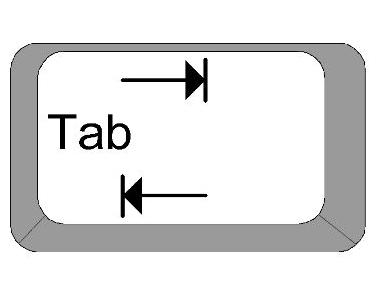
\includegraphics[scale=0.5]{../img/tab_key.jpg} para autocompletar las
  posibles rutas desde donde quiera que estes.
\item
  Escoge alguna (nuevamente usando la tecla tab para moverte entre las
  opciones). Si esto no funciona, teclea textualmente alguna de las
  rutas que ves.
\item
  Cierra la doble comilla y el paréntesis.
\item
  Teclea enter.
\item
  Debes encontrarte en la ruta elegida cuando tecleas \texttt{getwd()}.
\end{enumerate}

Con lo que acabamos de hacer, R buscará archivos o guardará archivos en
el folder \texttt{/home/animalito/study/}. En R también es posible
navegar a partir de el directorio de trabajo. Como siempre,

\begin{itemize}
\itemsep1pt\parskip0pt\parsep0pt
\item
  ``../un\_archivo.R'' le indica a R que busque un folder arriba del
  actual directorio de trabajo por el archivo \emph{un\_archivo.R}.
\item
  ``datos/otro\_archivo.R'' hace que se busque en el directorio de
  trabajo, dentro del folder \emph{datos} por el archivo
  \emph{otro\_archivo.R}
\end{itemize}

\begin{nota}
\textbf{Rutas relativas vs. Rutas absolutas\\}

El resultado que se muestra aquí al usar el comando \texttt{getwd()} depende de la computadora en la que se esta 
trabajando debido a que es una \textit{ruta absoluta}. Nota como es diferente la ruta 
que obtienes al correr el comando en tu consola de \texttt{R}. Eso es porque se trata 
de una ruta absoluta, es decir, es tal que da la ruta (\textit{path}) completo
al directorio en cuestión. Puedes accesar todos los directorios o archivos usando su ruta absoluta.\\

En investigación reproducible (\textit{reproducible research}), en investigación colaborativa o
incluso cuando trabajas en varias computadoras es una buena idea usar rutas relativas
en lugar de absolutas. Esto hace que el código sea menos dependiente de una estructura
de archivos o computadora en particular \parencite[][p. 67]{gandrud2013}. \\

En general, es \textit{buena práctica} configurar el código de un proyecto con rutas relativas.
En \texttt{R} en particular, cuando guardas un \texttt{Rmarkdown} y lo corres desde la línea de
comandos (o lo \textit{tejes} desde \texttt{RStudio}), la ruta que está fija -como si hubieras usado el comando \texttt{setwd()} es
en donde \textit{vive} ese archivo, es decir, el directorio en donde está guardado el mismo.\\

Desde cualquier \texttt{script} puedes llamar a otros usando este tipo de ruta como en 
el ejemplo anterior.
\end{nota}

\subsection{Ejemplos básicos}\label{ejemplos-basicos}

La consola permite hacer operaciones sobre números o caracteres (cuando
tiene sentido).

\begin{Shaded}
\begin{Highlighting}[]
\CommentTok{# Potencias, sumas, multiplicaciones}
\DecValTok{2}\NormalTok{^}\DecValTok{3} \NormalTok{+}\StringTok{ }\DecValTok{67} \NormalTok{*}\StringTok{ }\DecValTok{4} \NormalTok{-}\StringTok{ }\NormalTok{(}\DecValTok{45} \NormalTok{+}\StringTok{ }\DecValTok{5}\NormalTok{)}
\end{Highlighting}
\end{Shaded}

\begin{verbatim}
## [1] 226
\end{verbatim}

\begin{Shaded}
\begin{Highlighting}[]
\CommentTok{# Comparaciones}
\DecValTok{56} \NormalTok{>}\StringTok{ }\DecValTok{78} 
\end{Highlighting}
\end{Shaded}

\begin{verbatim}
## [1] FALSE
\end{verbatim}

\begin{Shaded}
\begin{Highlighting}[]
\DecValTok{34} \NormalTok{<=}\StringTok{ }\DecValTok{34}
\end{Highlighting}
\end{Shaded}

\begin{verbatim}
## [1] TRUE
\end{verbatim}

\begin{Shaded}
\begin{Highlighting}[]
\DecValTok{234} \NormalTok{<}\StringTok{ }\DecValTok{345}
\end{Highlighting}
\end{Shaded}

\begin{verbatim}
## [1] TRUE
\end{verbatim}

\begin{Shaded}
\begin{Highlighting}[]
\StringTok{"hola"} \NormalTok{==}\StringTok{ "hola"}
\end{Highlighting}
\end{Shaded}

\begin{verbatim}
## [1] TRUE
\end{verbatim}

\begin{Shaded}
\begin{Highlighting}[]
\StringTok{"buu"} \NormalTok{!=}\StringTok{ "yay"}
\end{Highlighting}
\end{Shaded}

\begin{verbatim}
## [1] TRUE
\end{verbatim}

\begin{Shaded}
\begin{Highlighting}[]
\CommentTok{# módulo}
\DecValTok{10} \NormalTok\StringTok{ }\DecValTok{4} 
\end{Highlighting}
\end{Shaded}

\begin{verbatim}
## [1] 2
\end{verbatim}

Estas operaciones también pueden ser realizadas entre vectores\footnote{Revisaremos
  más adelante con detalle la definición de vectores en la sección
  \ref{estructuras-de-datos}.}.

\begin{Shaded}
\begin{Highlighting}[]
\CommentTok{# Creamos un vector con entradas del -1 al 12 y lo asignamos a la variable x}
\NormalTok{x <-}\StringTok{ }\NormalTok{-}\DecValTok{1}\NormalTok{:}\DecValTok{12}
\CommentTok{# Lo vemos}
\NormalTok{x}
\end{Highlighting}
\end{Shaded}

\begin{verbatim}
##  [1] -1  0  1  2  3  4  5  6  7  8  9 10 11 12
\end{verbatim}

\begin{Shaded}
\begin{Highlighting}[]
\CommentTok{# Le sumamos 1 a todas las entradas}
\NormalTok{x +}\StringTok{ }\DecValTok{1}
\end{Highlighting}
\end{Shaded}

\begin{verbatim}
##  [1]  0  1  2  3  4  5  6  7  8  9 10 11 12 13
\end{verbatim}

\begin{Shaded}
\begin{Highlighting}[]
\CommentTok{# Multiplicamos por 2 cada entrada y le sumamos 3}
\DecValTok{2} \NormalTok{*}\StringTok{ }\NormalTok{x +}\StringTok{ }\DecValTok{3}
\end{Highlighting}
\end{Shaded}

\begin{verbatim}
##  [1]  1  3  5  7  9 11 13 15 17 19 21 23 25 27
\end{verbatim}

\begin{Shaded}
\begin{Highlighting}[]
\CommentTok{# Sacamos el módulo de cada entrada}
\NormalTok{x %%}\StringTok{ }\DecValTok{5} 
\end{Highlighting}
\end{Shaded}

\begin{verbatim}
##  [1] 4 0 1 2 3 4 0 1 2 3 4 0 1 2
\end{verbatim}

\subsection{Comandos útiles}\label{comandos-utiles}

Para enlistar los objetos que están en el espacio de trabajo

\begin{Shaded}
\begin{Highlighting}[]
\KeywordTok{ls}\NormalTok{()}
\end{Highlighting}
\end{Shaded}

\begin{verbatim}
## [1] "x"
\end{verbatim}

Para eliminar todos los objetos en un workspace

\begin{Shaded}
\begin{Highlighting}[]
\NormalTok{rm(list = ls(}\ErrorTok{))} \CommentTok{# se puede borrar solo uno, por ejemplo, nombrándolo}
\KeywordTok{ls}\NormalTok{()}
\end{Highlighting}
\end{Shaded}

\begin{verbatim}
## character(0)
\end{verbatim}

También se puede utilizar/guardar la historia de comandos utilizados

\begin{Shaded}
\begin{Highlighting}[]
\KeywordTok{history}\NormalTok{()}
\KeywordTok{history}\NormalTok{(}\DataTypeTok{max.show =} \DecValTok{5}\NormalTok{)}
\KeywordTok{history}\NormalTok{(}\DataTypeTok{max.show =} \OtherTok{Inf}\NormalTok{) }\CommentTok{# Muestra toda la historia}

\CommentTok{# Se puede salvar la historia de comandos a un archivo}
\KeywordTok{savehistory}\NormalTok{(}\DataTypeTok{file =} \StringTok{"mihistoria"}\NormalTok{) }\CommentTok{# Por default, R ya hace esto }
\CommentTok{# en un archivo ".Rhistory"}

\CommentTok{# Cargar al espacio de trabajo actual (current workspace) una }
\CommentTok{# historia de comandos en particular}
\KeywordTok{loadhistory}\NormalTok{(}\DataTypeTok{file =} \StringTok{"mihistoria"}\NormalTok{)}
\end{Highlighting}
\end{Shaded}

Es posible también guardar el workspace -en forma completa- en un
archivo con el comando \texttt{save.image()} a un archivo con extensión
\emph{.RData}. Puedes guardar una lista de objetos específica a un
archivo \emph{.RData}. Por ejemplo:

\begin{Shaded}
\begin{Highlighting}[]
\NormalTok{x <-}\StringTok{ }\DecValTok{1}\NormalTok{:}\DecValTok{12}
\NormalTok{y <-}\StringTok{ }\DecValTok{3}\NormalTok{:}\DecValTok{45}
\NormalTok{save(x, y, file = }\StringTok{"ejemplo.RData"}\ErrorTok{)} \CommentTok{#la extensión puede ser arbitraria.}
\end{Highlighting}
\end{Shaded}

Después puedo cargar ese archivo. Prueba hacer:

\begin{Shaded}
\begin{Highlighting}[]
\KeywordTok{rm}\NormalTok{(}\DataTypeTok{list =} \KeywordTok{ls}\NormalTok{()) }\CommentTok{# limpiamos workspace}
\NormalTok{load(file = }\StringTok{"ejemplo.RData"}\ErrorTok{)} \CommentTok{#la extensión puede ser arbitraria.}
\KeywordTok{ls}\NormalTok{()}
\end{Highlighting}
\end{Shaded}

Nota como los objetos preservan el nombre con el que fueron guardados.

\section{Paquetes (\emph{libraries})}\label{paquetes-libraries}

R puede hacer muchos análisis estadísticos y de datos. Las diferentes
capacidades están organizadas en paquetes o librerías. Con la
instalación estándar resumida en la sección \ref{instalacion}, se
instalan también los paquetes más comunes (también llamado el
\emph{base} o R-básico). Para obtener una lista de todos los paquetes
instalados se puede utilizar el comando \texttt{library()} en la consola
o en un script.

Existen una gran cantidad de paquetes disponibles además de los
incluidos por omisión (\emph{default}).

\subsection{CRAN}\label{cran}

\emph{Comprehensive R Archive Network} \parencite{cran} es una colección
de sitios que contienen exactamente el mismo material, es decir, son
espejos (\emph{mirrors}) de las distribuciones de R, las extensiones, la
documentación y los binarios. El master de CRAN está en
Wirtschaftsuniversität Wien en Austria. Éste se ``espeja''
(\emph{mirrors}) en forma diaria a muchos sitios alrededor del mundo. En
la \href{https://cran.r-project.org/mirrors.html}{lista de espejos} se
puede ver que para México están disponibles el espejo del ITAM, del
Colegio de Postgraduados (Texcoco) y Jellyfish Foundation
\parencite{cran}.

Los espejos son importantes pues, cada vez que busquen instalar
paquetes, se les preguntará qué espejo quieren utilizar para la sesión
en cuestión. Del espejo que selecciones, será del cuál R \emph{bajará}
el binario y la documentación.

Del CRAN es que se obtiene la última versión oficial de R. Diario se
actualizan los espejos. Para más detalles consultar el
\href{https://cran.r-project.org/doc/FAQ/R-FAQ.html}{FAQ}.

Para contribuir un paquete en CRAN se deben seguir las instrucciones
\href{https://cran.r-project.org/web/packages/policies.html}{aquí}.

\subsection{Github}\label{github}

Git es un controlador de versiones muy popular para desarrollar
software. Cuando se combina con \href{https://github.com/}{GitHub} se
puede compartir el código con el resto de la comunidad. Éste controlador
de versiones es el más popular entre los que contribuyen a R. Muchos
problemas a los que uno se enfrenta alguien ya los desarrolló y no
necesariamente publicó el paquete en CRAN. Para instalar algún paquete
desde GitHub, se pueden seguir las instrucciones siguientes

\begin{Shaded}
\begin{Highlighting}[]
\KeywordTok{install.packages}\NormalTok{(}\StringTok{"devtools"}\NormalTok{)}
\NormalTok{devtools::}\KeywordTok{install_github}\NormalTok{(}\StringTok{"username/packagename"}\NormalTok{)}
\end{Highlighting}
\end{Shaded}

Donde \texttt{username} es el usuario de Github y \texttt{packagename}
es el nombre del repositorio que contiene el paquete. Cuidado, no todo
repositorio en GitHub es un paquete. Para más información ver el
capítulo \href{http://r-pkgs.had.co.nz/git.html}{Git and GitHub} en
\textcite{wickham2015r}.

\subsection{Otras fuentes}\label{otras-fuentes}

Otros lugares en donde es común que se publiquen paquetes es en
\href{https://www.bioconductor.org/}{Bioconductor} un projecto de
software para la comprensión de datos del genoma humano.

\section{Paquetes recomendados}\label{paquetes-recomendados}

Hay muchísimas librerías y lo recomendable es, dado un problema y un
modelo para resolverlo, revisar si alguien ya implementó el método en
algunas de las fuentes de paquetes mencionadas antes.

Para mantener orden en los paquetes descargados puede ser útil utilizar
el \textcite{pacman} pues provee de herramientas para instalar paquetes
en una forma un poco más sencilla que usando la función
\texttt{install.packages}.

En particular, la función \texttt{p\_load} permite instalar, cargar y
actualizar uno o varios paquetes.

Si queremos instalar varios paquetes usando las herramientas del R
básico (\emph{base}) \parencite{rbase} haríamos algo como
\parencite[ejemplo tomado de][en la viñeta de intrducción al paquete]{pacman}:

\begin{Shaded}
\begin{Highlighting}[]
\NormalTok{packs <-}\StringTok{ }\KeywordTok{c}\NormalTok{(}\StringTok{"XML"}\NormalTok{, }\StringTok{"devtools"}\NormalTok{, }\StringTok{"RCurl"}\NormalTok{, }\StringTok{"fakePackage"}\NormalTok{, }\StringTok{"SPSSemulate"}\NormalTok{)}
\NormalTok{success <-}\StringTok{ }\KeywordTok{suppressWarnings}\NormalTok{(}\KeywordTok{sapply}\NormalTok{(packs, require, }\DataTypeTok{character.only =} \OtherTok{TRUE}\NormalTok{))}
\KeywordTok{install.packages}\NormalTok{(}\KeywordTok{names}\NormalTok{(success)[!success])}
\KeywordTok{sapply}\NormalTok{(}\KeywordTok{names}\NormalTok{(success)[!success], require, }\DataTypeTok{character.only =} \OtherTok{TRUE}\NormalTok{)}
\end{Highlighting}
\end{Shaded}

Con \texttt{pacman::p\_load} la tarea se reduce a:

\begin{Shaded}
\begin{Highlighting}[]
\NormalTok{pacman::}\KeywordTok{p_load}\NormalTok{(XML, devtools, RCurl, fakePackage, SPSSemulate)}
\end{Highlighting}
\end{Shaded}

\begin{curiosidad}
Nota como se puede llamar a una función por su nombre \texttt{p\_load} una vez que 
ya cargamos el paquete en el cuál esa función está guardada con el comando \texttt{library(pacman)}
o podemos llamarla directamente utilizando la convención \texttt{paquete::funcion}, en este caso,
\texttt{pacman::p\_load}.
\end{curiosidad}

Para instalar \texttt{pacman} escribe:

\begin{Shaded}
\begin{Highlighting}[]
\KeywordTok{install.packages}\NormalTok{(}\StringTok{"pacman"}\NormalTok{)}
\end{Highlighting}
\end{Shaded}

Algunos paquetes se encuentran en desarrollo. En particular, si se
encuentran en \texttt{github} pueden descargarse usando la función
\texttt{pacman::p\_install\_gh('usuario/repositorio')}.

A continuación, hay una lista de paquetes que se recomienda descargar o
revisar para tener a la mano herramientas diversas útiles para el
trabajo del científico de datos. La lista no es comprensiva pues hay un
gran número de paquetes útiles.

\begin{Shaded}
\begin{Highlighting}[]
\CommentTok{# Para cargar datos al ambiente de trabajo (data load)}
\NormalTok{pacman::}\KeywordTok{p_load}\NormalTok{(RODBC, RMySQL, RPostgreSQL, RSQLite, foreign, Rpostgres, haven}
               \NormalTok{, readr)}
\NormalTok{pacman::}\KeywordTok{p_install_gh}\NormalTok{(}\StringTok{"hadley/readxl"}\NormalTok{)}
\NormalTok{pacman::}\KeywordTok{p_install_gh}\NormalTok{(}\StringTok{"rstats-db/RPostgres"}\NormalTok{)}

\CommentTok{# Para manipular datos (data manipulation)}
\NormalTok{pacman::}\KeywordTok{p_load}\NormalTok{(plyr, dplyr, data.table, tidyr, stringr, lubridate, gsubfn)}

\CommentTok{# Para visualizar datos (data visualization)}
\NormalTok{pacman::}\KeywordTok{p_load}\NormalTok{(ggplot2, graphics, ggvis)}
\NormalTok{pacman::}\KeywordTok{p_install_gh}\NormalTok{(}\StringTok{"RcppCore/Rcpp"}\NormalTok{)}
\NormalTok{pacman::}\KeywordTok{p_install_gh}\NormalTok{(}\StringTok{"rstats-db/DBI"}\NormalTok{)}
\NormalTok{pacman::}\KeywordTok{p_install_gh}\NormalTok{(}\StringTok{'ramnathv/htmlwidgets'}\NormalTok{)}
\NormalTok{pacman::}\KeywordTok{p_install_gh}\NormalTok{(}\StringTok{'rstudio/leaflet'}\NormalTok{)}
\NormalTok{pacman::}\KeywordTok{p_install_gh}\NormalTok{(}\StringTok{'bwlewis/rthreejs'}\NormalTok{)}
\NormalTok{pacman::}\KeywordTok{p_install_gh}\NormalTok{(}\StringTok{'htmlwidgets/sparkline'}\NormalTok{)}
\NormalTok{pacman::}\KeywordTok{p_load}\NormalTok{(dygraphs, DT, DiagrammeR, networkD3, googleVis)}

\CommentTok{# Para modelar (data modelling)}
\NormalTok{pacman::}\KeywordTok{p_load}\NormalTok{(car, mgcv, lme4, nlme, randomForest, multcomp, vcd, glmnet, survival, caret)}

\CommentTok{# Para generar reportes (reports)}
\NormalTok{pacman::}\KeywordTok{p_load}\NormalTok{(shiny, xtable, knitr, rmarkdown)}

\CommentTok{# Para trabajar con datos espaciales (spatial data)}
\NormalTok{pacman::}\KeywordTok{p_load}\NormalTok{(sp, maptools, maps, ggmap, rgdal)}

\CommentTok{# Para trabajo con series de tiempo (time series)}
\NormalTok{pacman::}\KeywordTok{p_load}\NormalTok{(zoo, quantmod)}

\CommentTok{# Para escribir código de alto rendimiento en R (High performance R code)}
\NormalTok{pacman::}\KeywordTok{p_load}\NormalTok{(Rcpp, parallel)}

\CommentTok{# Trabajar con la web }
\NormalTok{pacman::}\KeywordTok{p_load}\NormalTok{(XML, jsonlite, httr)}

\CommentTok{# Para escribir paquetes en R}
\NormalTok{pacman::}\KeywordTok{p_load}\NormalTok{(devtools, testthat, roxygen2)}
\end{Highlighting}
\end{Shaded}

\section{Scripting}\label{scripting}

R es un intérprete. Utiliza un ambiente basado en línea de comandos. Por
ende, es necesario escribir la secuencia de comandos que se desea
realizar a diferencia de otras herramientas en donde es posible utlizar
el mouse o menús.

Aunque los comandos pueden ser ejecutados directamente en consola una
única vez, también es posible guardarlos en archivos conocidos como
\emph{scripts}. Típicamente, utilizamos la extensión \textbf{.R} o
\textbf{.r}. En RStudio \parencite{rstudio}, \texttt{CTRL + SHIFT + N}
abre inmediatamente un nuevo editor en el panel superior izquierdo.

En RStudio, por ejemplo, se puede \emph{ir editando} el script y
corriendo los comandos línea por línea con \texttt{CTRL + ENTER}. Esto
también aplica para \emph{correr} una selección del texto
editable\footnote{RStudio tiene muchos
  \href{https://support.rstudio.com/hc/en-us/articles/200711853-Keyboard-Shortcuts}{atajos
  de teclado} que facilitan el trabajo.}.

Es posible también correr todo el script

\begin{Shaded}
\begin{Highlighting}[]
\KeywordTok{source}\NormalTok{(}\StringTok{"foo.R"}\NormalTok{)}
\end{Highlighting}
\end{Shaded}

O con el atajo \texttt{CTRL + SHIFT + S} en RStudio.

Para enlistar algunos shortcuts comunes en RStudio presiona
\texttt{ALT + SHIFT + K}.

De la misma manera, si utilizas \texttt{Emacs + ESS}
\parencite{rossini2004ess}, existen múltiples atajos de teclado para
realizar todo mucho más eficientemente. Estudiarlos no es tiempo
perdido.

\section{Ayuda y documentación}\label{ayuda-y-documentacion}

\texttt{R} tiene mucha documentación. Dado que es imposible recordar
todas las funciones o cómo utilizar todo lo que ya está hecho, es
necesario aprender a leerla. Desde la consola se puede accesar a la
misma.

Para ayuda general,

\begin{Shaded}
\begin{Highlighting}[]
\KeywordTok{help.start}\NormalTok{()}
\end{Highlighting}
\end{Shaded}

Para la \textbf{ayuda de una función en especifico}, por ejemplo, si se
quiere graficar algo y sabemos que existe la funcion \texttt{plot}
podemos consultar fácilmente la ayuda.

\begin{Shaded}
\begin{Highlighting}[]
\KeywordTok{help}\NormalTok{(plot)}
\CommentTok{# o tecleando directamente}
\NormalTok{?plot}
\end{Highlighting}
\end{Shaded}

El segundo ejemplo se puede extender para buscar esa función en todos
los paquetes que tengo instalados en mi ambiente al escribir
\texttt{??plot}.

A veces, es útil ver el \textbf{cuerpo de una función}. Esta tarea no
necesariamente es trivial. Para funciones generadas por el usuario, usa

\begin{Shaded}
\begin{Highlighting}[]
\NormalTok{xx <-}\StringTok{ }\NormalTok{function(x) x^}\DecValTok{2}
\KeywordTok{body}\NormalTok{(xx)}
\end{Highlighting}
\end{Shaded}

\begin{verbatim}
## x^2
\end{verbatim}

\begin{Shaded}
\begin{Highlighting}[]
\CommentTok{# o simplemente imprimir el objeto en donde guardamos la función}
\NormalTok{xx}
\end{Highlighting}
\end{Shaded}

\begin{verbatim}
## function(x) x^2
\end{verbatim}

También funciona para algunas funciones de paquete, por ejemplo
\texttt{rename}:

\begin{Shaded}
\begin{Highlighting}[]
\KeywordTok{library}\NormalTok{(plyr)}
\KeywordTok{body}\NormalTok{(rename)}
\end{Highlighting}
\end{Shaded}

\begin{verbatim}
## {
##     names(x) <- revalue(names(x), replace, warn_missing = warn_missing)
##     duplicated_names <- names(x)[duplicated(names(x))]
##     if (warn_duplicated && (length(duplicated_names) > 0L)) {
##         duplicated_names_message <- paste0("`", duplicated_names, 
##             "`", collapse = ", ")
##         warning("The plyr::rename operation has created duplicates for the ", 
##             "following name(s): (", duplicated_names_message, 
##             ")", call. = FALSE)
##     }
##     x
## }
\end{verbatim}

Para plot, en cambio, al usar la función \texttt{body} se ve:

\begin{Shaded}
\begin{Highlighting}[]
\KeywordTok{body}\NormalTok{(plot)}
\end{Highlighting}
\end{Shaded}

\begin{verbatim}
## UseMethod("plot")
\end{verbatim}

Esto es porque \texttt{plot} es una función genérica (S3) que tiene
métodos para distintas clases de objetos. En esos casos, primero debemos
usar la función \texttt{methods} para enlistar los métodos que tiene esa
función.

\begin{Shaded}
\begin{Highlighting}[]
\KeywordTok{methods}\NormalTok{(plot)}
\end{Highlighting}
\end{Shaded}

\begin{verbatim}
##  [1] plot.acf*           plot.data.frame*    plot.decomposed.ts*
##  [4] plot.default        plot.dendrogram*    plot.density*      
##  [7] plot.ecdf           plot.factor*        plot.formula*      
## [10] plot.function       plot.hclust*        plot.histogram*    
## [13] plot.HoltWinters*   plot.isoreg*        plot.lm*           
## [16] plot.medpolish*     plot.mlm*           plot.ppr*          
## [19] plot.prcomp*        plot.princomp*      plot.profile.nls*  
## [22] plot.raster*        plot.spec*          plot.stepfun       
## [25] plot.stl*           plot.table*         plot.ts            
## [28] plot.tskernel*      plot.TukeyHSD*     
## see '?methods' for accessing help and source code
\end{verbatim}

Si tiene asteriscos, significa que la función para ese método en
particular no viene directamente del espacio de nombres del paquete
pero, de cualquier forma, lo podemos pedir usando la
\texttt{función getAnywhere} para cualquiera de los métodos que se
desplegaron:

\begin{Shaded}
\begin{Highlighting}[]
\KeywordTok{getAnywhere}\NormalTok{(plot.density)}
\end{Highlighting}
\end{Shaded}

\begin{verbatim}
## A single object matching 'plot.density' was found
## It was found in the following places
##   registered S3 method for plot from namespace stats
##   namespace:stats
## with value
## 
## function (x, main = NULL, xlab = NULL, ylab = "Density", type = "l", 
##     zero.line = TRUE, ...) 
## {
##     if (is.null(xlab)) 
##         xlab <- paste("N =", x$n, "  Bandwidth =", formatC(x$bw))
##     if (is.null(main)) 
##         main <- deparse(x$call)
##     plot.default(x, main = main, xlab = xlab, ylab = ylab, type = type, 
##         ...)
##     if (zero.line) 
##         abline(h = 0, lwd = 0.1, col = "gray")
##     invisible(NULL)
## }
## <bytecode: 0x1ea9370>
## <environment: namespace:stats>
\end{verbatim}

Nota como el método \texttt{plot.density} viene del paquete
\texttt{stats}
\footnote{Hay otro tipo de funciones en las accesar al código fuente no se pueda con los métodos descritos. Para ello, es útil revisar la sección "old-school object-oriented programming in R" \parencite[][p.131-133]{adler2010r} o las secciones dedicadas a los objetos S3 y S4 en \textcite{wickham2014advanced}.}.

La documentación normalmente se acompaña de \textbf{ejemplos}. Para
\emph{correr} los ejemplos sin necesidad de copiar y pegar, prueba

\begin{Shaded}
\begin{Highlighting}[]
\KeywordTok{example}\NormalTok{(plot)}
\end{Highlighting}
\end{Shaded}

Para búsquedas más comprensivas, se puede buscar de otras maneras:

\begin{Shaded}
\begin{Highlighting}[]
\KeywordTok{apropos}\NormalTok{(}\StringTok{"foo"}\NormalTok{) }\CommentTok{# Enlista todas las funciones que contengan la cadena "foo"}
\KeywordTok{RSiteSearch}\NormalTok{(}\StringTok{"foo"}\NormalTok{) }\CommentTok{# Busca por la cadena "foo" en todos los manuales de ayuda }
\CommentTok{# y listas de distribución.}
\end{Highlighting}
\end{Shaded}

\section{Optimizando}\label{optimizando}

Es común que muy pronto nos encontremos con limitaciones al poder de
cómputo y rapidez con el que R procesa los datos. Hay operaciones
intensivas como, por ejemplo, la inversión de matrices (qr) o el
análisis por componentes principales (svd). Incluso una selección de
variables (\emph{back/forward selection}) usando una simple regresión
lineal sobre múltiples regresores puede llevar un tiempo de cómputo de
horas/días o no terminar.

Una de las manera más rápidas de mejorar el performance de \texttt{R} es
instalando las librerías de álgebra lineal que puede utilizar el
software para hacer las operaciones más rápido.

Para mucho (demasiado) detalle al respecto, referirse a la comparación
de performance en \textcite{eddelbuettel2010} o al paquete del mismo
autor \textcite{gcbd}.

Para la parte práctica de todo esto, referirse a
\href{http://brettklamer.com/diversions/statistical/faster-blas-in-r/}{este
blog} para instalar las librerías apropiadas para BLAS y Lapack
\parencite{blasinr}. Para una comparación bastante práctica de las
diferentes versiones de esas librerías, ver
\href{http://blog.nguyenvq.com/blog/2014/11/10/optimized-r-and-python-standard-blas-vs-atlas-vs-openblas-vs-mkl/}{aquí}
\parencite{optimizedr}.

\end{document}
